\documentclass[12pt]{article}
\usepackage{color}
\usepackage[usenames,dvipsnames,svgnames,table]{xcolor}
\definecolor{dark-red}{rgb}{0.7,0.1,0.1} 
\definecolor{dark-blue}{rgb}{0,0,0.7} 
\usepackage[linkcolor=dark-red,
            colorlinks=true,
            urlcolor=dark-blue,
            pdfstartview={XYZ null null 1.00},
            pdfauthor={Gaurav Sood, gsood07@gmail.com},
            citecolor=dark-red,
            bookmarks=false,
            pdfborder={0 0 0},
            pdftitle={The Review}]{hyperref}
            
\usepackage{amsfonts,amssymb,amsbsy,amsmath,amsxtra}

\usepackage[letterspace=1000]{microtype}
\usepackage{libertine}
\usepackage[T1]{fontenc}

\usepackage{indentfirst}
\usepackage{setspace} % To set line spacing
\usepackage{multirow}

\usepackage{verbatim}

\usepackage[multiple]{footmisc}
\usepackage{fancyvrb}

\usepackage{longtable}

\usepackage[margin=1in]{geometry}
\usepackage{graphicx}

\raggedright
\parindent=1.5em % <- or whatever indent you want

\usepackage{natbib}
\usepackage{url}
\begin{comment}

setwd(paste0(githubdir, "/meta_apsr/ms/"))	
tools::texi2dvi("the_review.tex", pdf=TRUE, clean=TRUE)	
setwd(paste0(githubdir, "/meta_apsr/"))

\end{comment}

\begin{document}
\title{\vspace{-.5cm}\normalsize{The Review: Production and Consumption of APSR Articles}}
\author{\vspace{.2cm}\\\normalsize{Gaurav Sood}\\\href{mailto:gsood07@gmail.com}{\small{gsood07@gmail.com}}\vspace{.3cm}\\}
\date{\normalsize{October 3rd, 2015}}
\maketitle
\begin{center}
\textbf{NB:} Preliminary draft. Please do not cite without permission.
\end{center}
\vspace{.4cm}
\doublespacing

Scientific production is affected by a variety of variables that have little to do with science. For instance, investment in research is correlated with commercialization lags --- greater the lags, lower the investment \citep{budish2013firms}.\footnote{The article posits that later stage cancer drugs have smaller commercialization lags. It isn't clear why. But the general point likely holds.} On the flip side, minor changes to how research is delivered can have astonishingly large consequences for consumption of research. For instance, papers listed first get a 27\% more citations than papers listed at other locations.\footnote{ See \href{http://www.npr.org/2015/07/15/423101360/no-1-with-a-bullet-point-to-get-research-cited-make-sure-its-listed-first}{http://www.npr.org/2015/07/15/423101360/no-1-with-a-bullet-point-to-get-research-cited-make-sure-its-listed-first}.} More generally, a broad range of factors, from availability of funding to fads to various parts of the scientific paper production pipeline, including, the number of articles editors must review, the incentives to be nice to the author, likely affect what topic is researched, the quality of the research, who produces the research, and how many read it. 

Using an original dataset of rich meta data on all articles published in the The American Political Science Review (APSR), the preeminent political science journal since its inception, nearly a hundred years ago, I shed light on some of these issues.\footnote{The data and scripts to acquire, process and analyze the data can be downloaded from \href{https://github.com/soodoku/meta_apsr}{https://github.com/soodoku/meta\_apsr}.} In particular, I study whether, like top economic journals, over time The Review is publishing fewer articles \citep{card2013nine, card2014page}. I find that the number of articles published by the APSR has increased over time, though it has plateaued over the last thirty or so years.

Next, I investigate two particular aspects of production --- co-authorship and gender of authors. For a variety of reasons --- ease of co-authorship, greater differentiation in skills, greater complexity of projects --- the proportion of co-authored articles in a variety of fields is on the rise \citep{barnett1988rising, card2013nine, cunningham1997authorship}. I study whether that is true for the APSR. Expectedly, I find that co-authorship rates have increased significantly. Second, I estimate the proportion of women per published articles in the APSR over time. (Pairing it with American Political Science Association membership data would provide one (unsatisfactory) way of getting an estimate of gender bias.   )

Next, I move to study consumption using consumption. I find that both the abstract views and full-text views follow the well-known power law distribution, with a few articles receiving a lot of views and most articles receiving no views. I end by doing something fun. Some previous analyses have suggested that paper titles have gotten longer over time.\footnote{See \href{http://datacolada.org/2013/12/04/titleogy/}{http://datacolada.org/2013/12/04/titleogy/}} I check whether this is true for the APSR. I find that it is.

\section*{Data and Results} 
In total, there are 30,235 editor's notes, rejoinders, articles, research notes, book reviews and other miscellanea that have been published in the APSR. (The number refers to the total number of unique document object identifiers.) Of these, I exclude all editor's notes, book reviews, etc. from consideration. This pares down the data to 4,385 articles, which serves as the final dataset. The data include information on the number of pages in each issue (volume), the title, the abstract and the pages spanned by each article, names and institutional affiliation of the authors, and total number of times the abstract, and full-text of the article was viewed. To these data, I add imputed gender of the authors --- proportion of people with the name who were women --- using the R Package {\tt gender} \citet{lincoln2015}.\footnote{Given the age of the author is unknown and given time can be correlated with gender distribution of a name, I assume that the age of an author is uniformly distributed between 25 and 65. This is unsatisfactory still but a variety of trials using variety of ranges of years yields very similar answers.}

Over the past 100 or so years, article length has shown marked variability (see Figure~\ref{fig:pages}). There is a marked see-saw pattern in the average length of the article, but unlike top economics journals we don't see a marked trend towards longer articles. (It is very likely, however, that the length of online appendices has grown substantially.)

Over time, the number of articles per issue has shown a sharp increase --- over 100 years, the number of articles has more than doubled (see Figure~\ref{fig:narticles}). (Though, over the past thirty or so years, the number of articles per issue has remained steady.) Given the two facts --- similar article length, increase in number of articles --- it is obvious that pages per issue would have increased. And so we find (see Figure~\ref{fig:issue}). 

Looking at production, I tallied two features: number of authors per article over time, and proportion of female authors per article over time. Like with other sciences, co-authorship is on the rise. Though, solo authored papers still make a sizable proportion of publications in the APSR, the modal publication today has two authors (see Figure~\ref{fig:nauthors}).

The data on proportion of women authors per article is distressing. While again the proportion of women on each article published in the APSR has been rising, the average article still has just 20\% female authors (see Figure~\ref{fig:women}).  

Flipping the lens and looking at two consumption metrics: number of abstract views and number of full-text views, provides a familiar power-law distribution. Most of the articles (abstracts) aren't viewed at all. And a small set of articles gets a lot of views (see Figures~\ref{fig:abstracts} and ~\ref{fig:fulltext}).

Lastly, some fun. Plotting the length of titles of APSR articles over time clearly shows that the titles have become longer over time. In fact, the average title length has increased by 50\% --- from an average of 50 to about 75 characters today.

\clearpage
\begin{center}
\large{Figures}
\end{center}

\begin{figure}[htbp]
\centering
\caption{Number of Pages per Article Over Time}
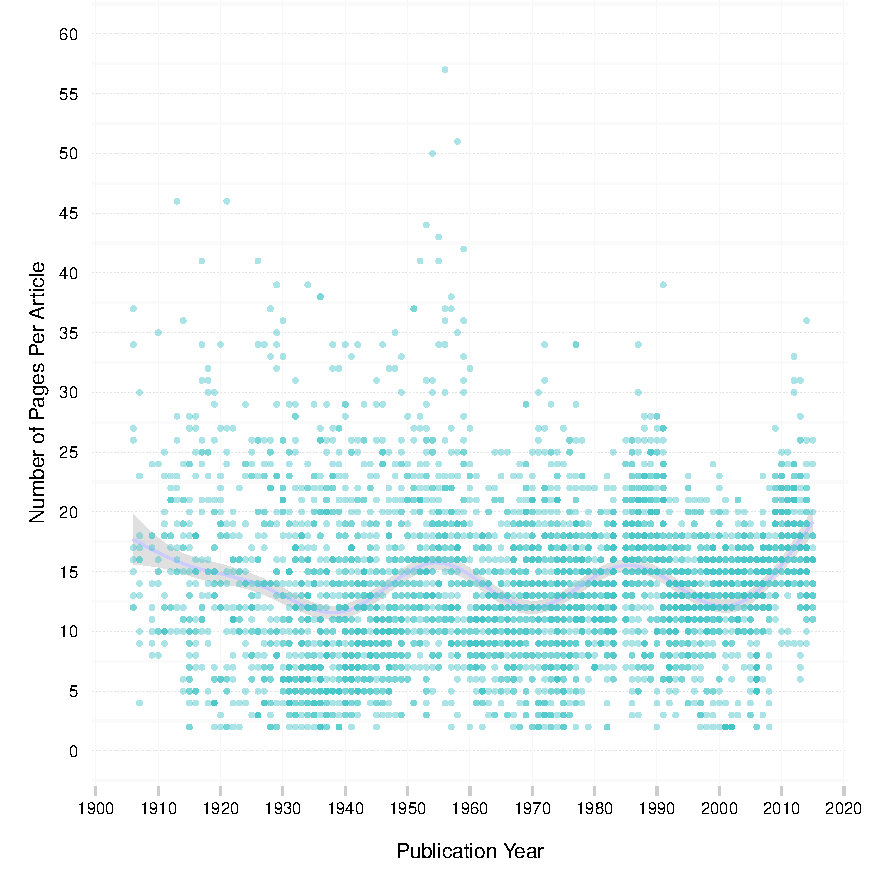
\includegraphics[scale=.85]{../figs/n_pages_per_article_over_time.pdf}
\label{fig:pages}
\end{figure}

\begin{figure}[htbp]
\centering
\caption{Number of Articles per Issue Over Time}
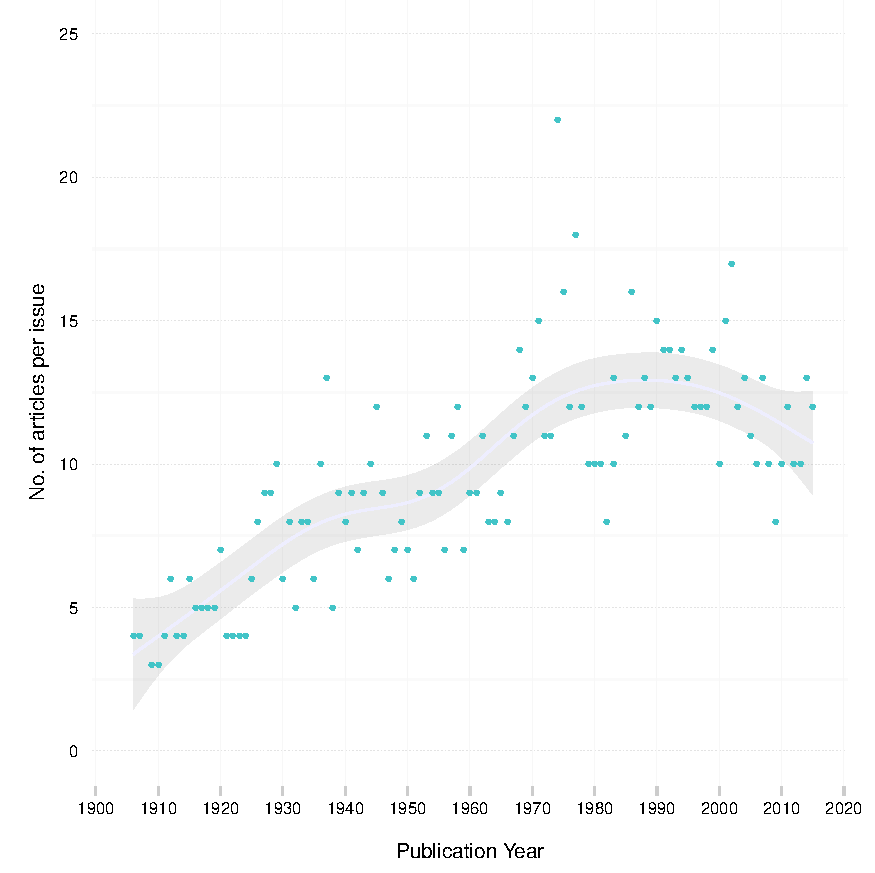
\includegraphics[scale=.85]{../figs/articles_per_issue_over_time.pdf}
\label{fig:narticles}
\end{figure}

\begin{figure}[htbp]
\centering
\caption{Pages per Issue Over time}
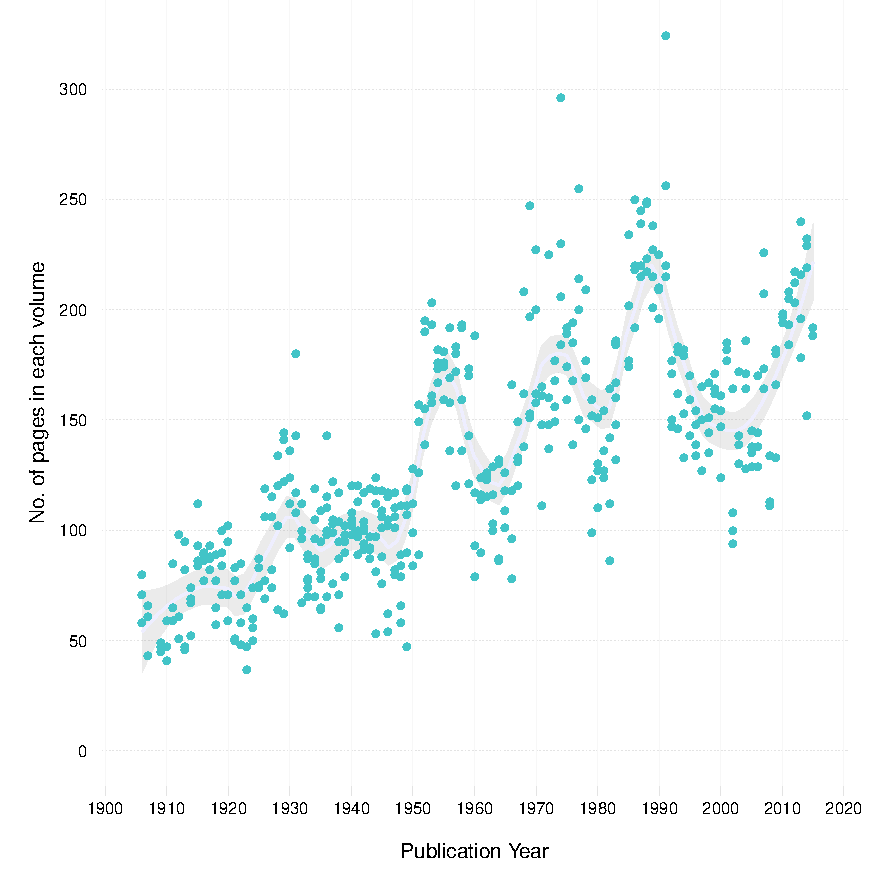
\includegraphics[scale=.85]{../figs/pages_per_issue_over_time.pdf}
\label{fig:issue}
\end{figure}

\begin{figure}[htbp]
\centering
\caption{Number of Authors per Article Over Time}
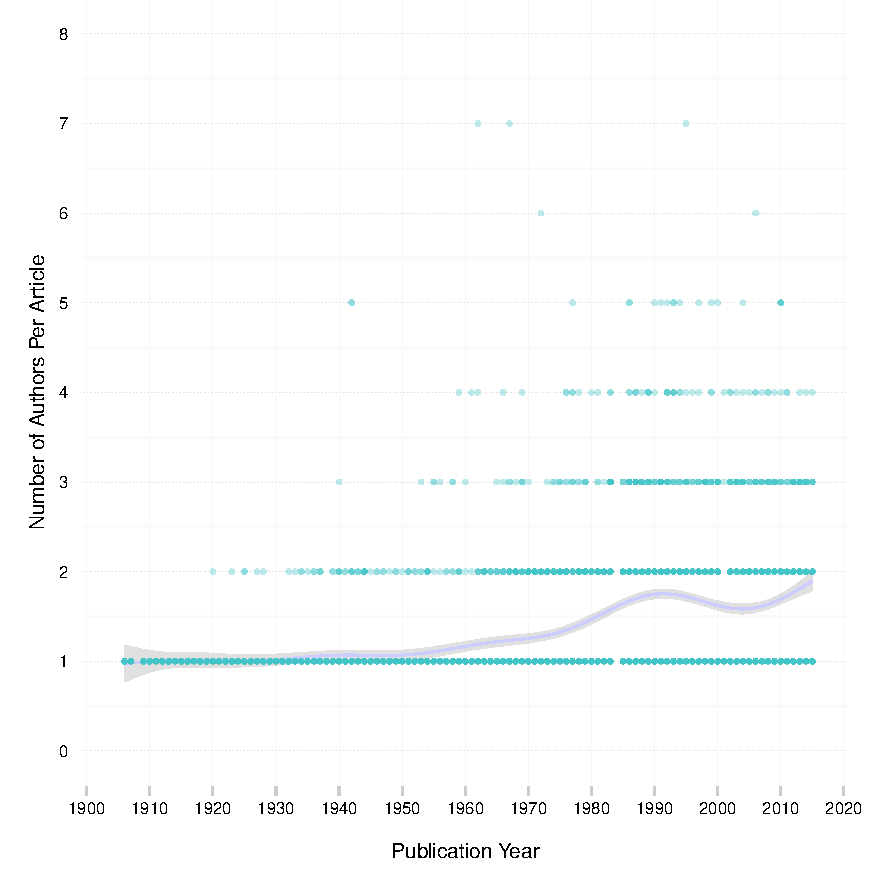
\includegraphics[scale=.85]{../figs/n_authors_per_article_over_time.pdf}
\label{fig:nauthors}
\end{figure}

\begin{figure}[htbp]
\centering
\caption{Proportion of Women Per Article Over Time}
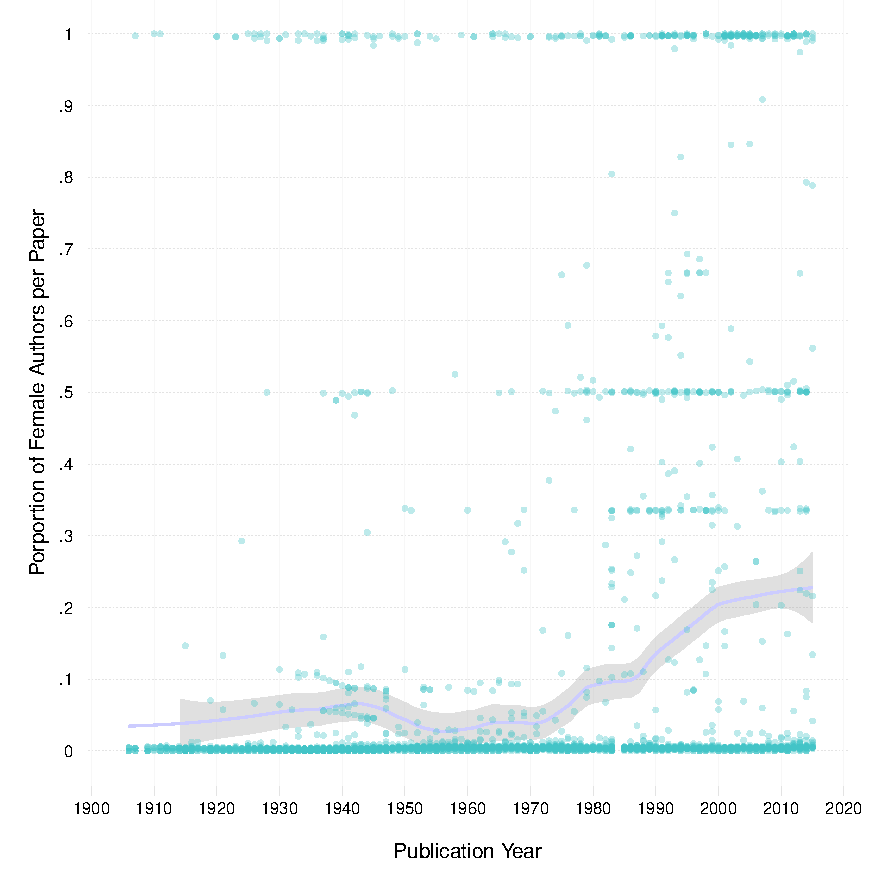
\includegraphics[scale=.85]{../figs/gender_authors_per_article_over_time.pdf}
\label{fig:women}
\end{figure}

\begin{figure}[htbp]
\centering
\caption{Abstract Views}
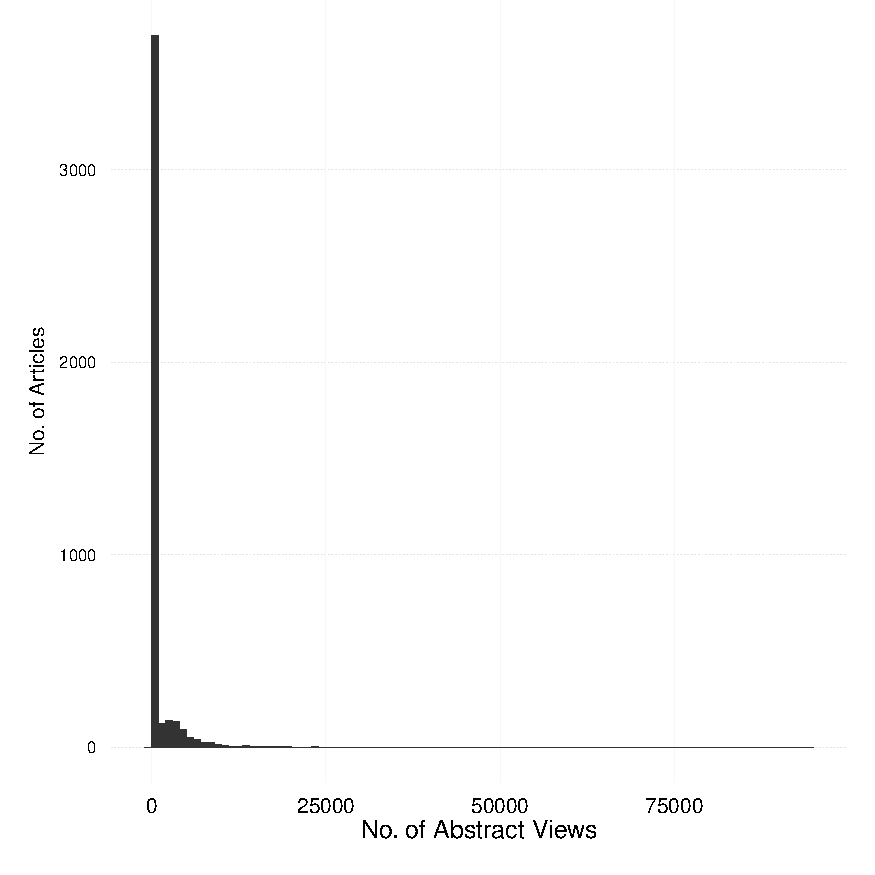
\includegraphics[scale=.85]{../figs/abstract_views.pdf}
\label{fig:abstracts}
\end{figure}

\begin{figure}[htbp]
\centering
\caption{Full-Text Views}
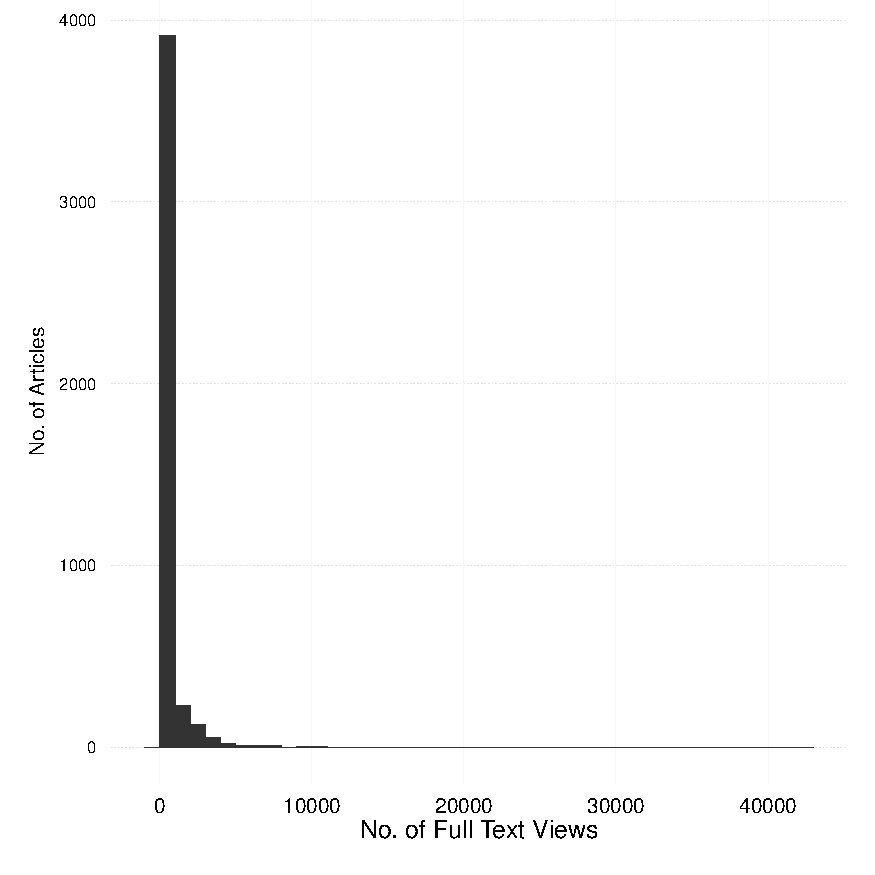
\includegraphics[scale=.85]{../figs/fulltext_views.pdf}
\label{fig:fulltext}
\end{figure}

\begin{figure}[htbp]
\centering
\caption{Title Length Over Time}
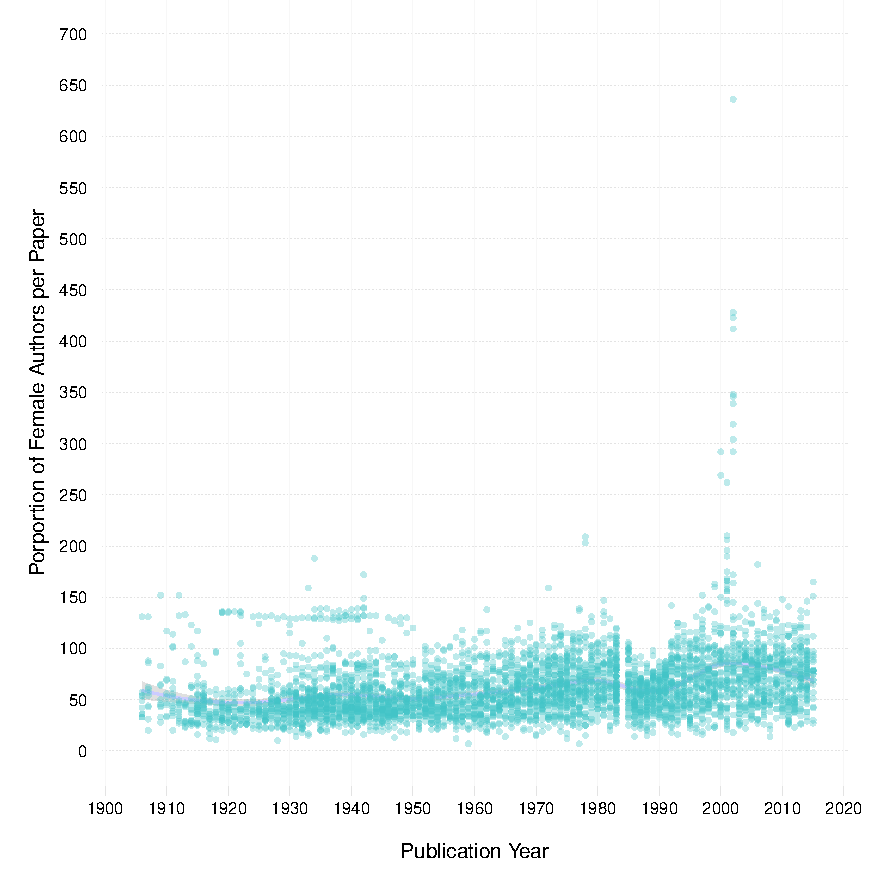
\includegraphics[scale=.85]{../figs/title_len_over_time.pdf}
\label{fig:fulltext}
\end{figure}

\clearpage
\bibliographystyle{apsr}
\bibliography{reviewbib}

\end{document}